\documentclass[../report.tex]{subfiles}
\begin{document}
    
    \begin{frame}[t]
        \frametitle{4a: Image Stats}
        \begin{normalsize}
            \begin{itemize}
                \setlength\itemsep{1em}
                
                \item[]{\fontsize{12pt}{12pt}\selectfont\textcolor{blue}{Min: 0.0 \\
Max: 255.0 \\
Mean: 119.12488932291667 \\
Standard Deviation: 57.09495205175706 \\
}}
                
            \end{itemize}
        \end{normalsize}
    \end{frame}

    \begin{frame}
        \frametitle{4b: Arithmetic Operation}
        \begin{figure}[!htb]
            \centering
            \frame{
\includegraphics[keepaspectratio,height=0.65\textheight,width=0.45\textwidth]{ps1-4-b-1}}
            \caption{ps1-4-b-1}
        \end{figure}
    \end{frame}

    \begin{frame}
        \frametitle{4c: Shifted Image}
        \begin{figure}[!htb]
            \centering
            \frame{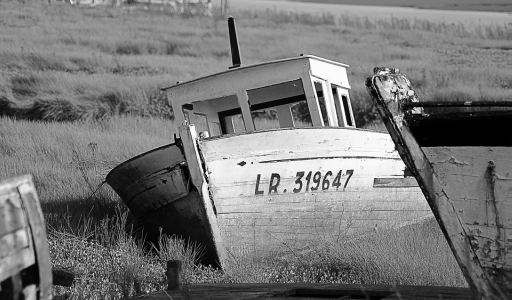
\includegraphics[keepaspectratio,height=0.65\textheight,width=0.45\textwidth]{ps1-4-c-1}}
            \caption{ps1-4-c-1}
        \end{figure}
    \end{frame}

    \begin{frame}
        \frametitle{4d: Difference Image}
        \begin{figure}[!htb]
            \centering
            \frame{
\includegraphics[keepaspectratio,height=0.65\textheight,width=0.45\textwidth]{ps1-4-d-1}}
            \caption{ps1-4-d-1}
        \end{figure}
    \end{frame}
    
\end{document}